\begin{frame}
The performance of rocket engines relies heavily on the flow of gases
through the nozzle. Therefore, a thorough understanding of flow and heat
transfer in rocket nozzles is essential for their design and
optimization. In this paper, we propose a methodology that utilizes
neural networks and singular value decomposition to reconstruct the
internal flow and heat transfer fields in a rocket nozzle. The
methodology involves two main steps. Firstly, we use both low and high
fidelity computational fluid dynamics (CFD) analyses to simulate the
flow of gases through the nozzle and predict the heat transfer.
Secondly, we decompose the data matrix generated from the CFD
simulations using singular value decomposition (SVD) and train a neural
network to learn the relationship between the dominant modes obtained
from the SVD of both fidelity simulations.The trained neural network can
then be used to reconstruct the flow and heat transfer fields from the
low fidelity solutions. The proposed methodology has been shown to
accurately predict fluid flows and, to some extent, temperature and heat
flux in the nozzle walls. The surrogate model developed using this
methodology has great potential for improving the design and
optimization of nozzle flows.
\end{frame}

\begin{frame}{Introduction}
\protect\hypertarget{introduction}{}
In the field of rocket propulsion, accurate prediction of heat transfer
in nozzle flow plays a critical role in designing and optimizing rocket
engines {[}@Zhang2011{]}. However, existing methods for predicting heat
transfer often suffer from high computational complexity, making them
impractical for engineering design purposes. To address this challenge,
we propose a flow reconstruction {[}@Lui2019; @Yu2019{]} technique that
combines order reduction using Singular Value Decomposition
(SVD){[}@Golub2013-ag{]} with neural network modeling
{[}@Brunton2019-ax{]}. While the individual techniques are not novel,
our approach offers a combination of these methods for accurate and
efficient prediction of internal flow and thermal fields in the nozzle,
leading to highly accurate fluid flow predictions. Furthermore, the use
of neural network modeling enhances the accuracy of our approach by
capturing the complex nonlinearities of the flow. Overall, our flow
reconstruction technique has the potential to significantly improve the
design and optimization of conjugate heat transfer CFD problems,
providing valuable insights into the underlying physical phenomena while
reducing computational complexity.
\end{frame}

\begin{frame}{Methodology}
\protect\hypertarget{methodology}{}
Flow reconstruction {[}@Yu2019{]} is a technique used to recover
high-fidelity computational fluid dynamics (CFD) simulations from
low-fidelity ones. This can be accomplished using neural networks and
singular value decomposition (SVD). The proposed methodology is
data-driven and consists of three main steps.

In the first step, the data is generated. To generate a set of high
fidelity simulations, the input parameters are varied to cover a wide
range of flow conditions. To generate a set of low fidelity simulations,
the resolution is reduced, the model is simplified, or a less accurate
numerical method is used. In the second step, both sets of simulations
are reduced to a set of basis functions coefficients using SVD, which
capture the dominant modes of variation in the flow fields. This allows
for a more efficient representation of the flow field and facilitates
the use of neural networks for flow reconstruction.

The final step of the proposed flow reconstruction technique involves
training a neural network to map the low-fidelity reduced simulations to
their corresponding high-fidelity counterparts. During the online
training stage, the neural network takes a set of low-fidelity basis
coefficients as input and generates a set of coefficients for the
high-fidelity reduced basis as output. Once trained, the neural network
can be used for inference in the offline stage. During inference, the
low-fidelity simulation in full space is projected onto the basis
coefficients using SVD. These coefficients are then used as input to the
trained neural network to predict the corresponding high-fidelity basis
coefficients. Finally, a reverse projection operation is performed on
the predicted coefficients to recover the high-fidelity simulation in
full space. Figure provides a schematic representation of this
reconstruction approach.

\begin{figure}
\hypertarget{fig:flow_chart}{%
\centering
\includegraphics{figures/inference.png}
\caption{Flow reconstruction inference flow
chart.}\label{fig:flow_chart}
}
\end{figure}

\begin{block}{Step 1: Data Generation using CFD Analysis}
\protect\hypertarget{step-1-data-generation-using-cfd-analysis}{}
In this work, we aim to develop a surrogate model that predicts the 2D
viscous airflow, temperature, and heat flux on the inner surface of a
nozzle, using only quasi-1D simulations. For the model to be useful for
design purposes, it must also be sensitive to geometrical parameters.
Therefore, we focus on two key design variables: the thickness of the
nozzle wall (\(t_w\)) and the shape of the nozzle wall, which is defined
by the y-coordinate of a Bezier control point (\(CP3_y\)), as shown in
Figure \protect\hyperlink{fig:nozzle_shape}{2}.

To begin, we use Latin Hypercube sampling (LHS) {[}@McKay1979{]} to
sample 30 design variables in the range provided in Table
\protect\hyperlink{tab:lhs}{1}, as shown in Figure
\protect\hyperlink{fig:lhs}{3}. We consider a set of \(N\) pairs of
design variables denoted as \(\Xi^i=\left\{t_w, CP3_y\right\}^i\). For
each pair, we collect a low-fidelity snapshot
(\(\mathbf{L}^i \in \mathbb{R}^{S_L}\)) and a high-fidelity snapshot
(\(\mathbf{H}^i \in \mathbb{R}^{S_H}\)) that contain the modeled
variables.

To store the low-fidelity and high-fidelity snapshots, we use two
matrices, denoted by \(\mathbf{A}_L\) and \(\mathbf{A}_H\),
respectively. The low-fidelity snapshots are stored in \(\mathbf{A}_L\)
according to Equation \protect\hyperlink{eq:A_L}{{[}eq:A\_L{]}}, while
the high-fidelity snapshots are stored in \(\mathbf{A}_H\) according to
Equation \protect\hyperlink{eq:A_H}{{[}eq:A\_H{]}}.

\[\mathbf{A}_L = \left[ \mathbf{L}^1 | \dots | \mathbf{L}^N\right]^{S_L \times N}     
\label{eq:A_L}\]

\[\mathbf{A}_H = \left[ \mathbf{H}^1 | \dots | \mathbf{H}^N\right]^{S_H \times N}
\label{eq:A_H}\]

\begin{figure}
\hypertarget{fig:nozzle_shape}{%
\centering
\includegraphics{figures/nozzle_shape.pdf}
\caption{Nozzle shape defined by the thickness of the wall (\(t_w\)) and
the y-coordinate of a Bezier control point
(\(CP3_y\)).}\label{fig:nozzle_shape}
}
\end{figure}

\begin{figure}
\hypertarget{fig:lhs}{%
\centering
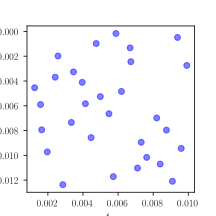
\includegraphics{figures/lhs_sampling.pdf}
\caption{Latin Hypercube Sampling of 30 design variables within the
sampling ranges given in Table
\protect\hyperlink{tab:lhs}{1}.}\label{fig:lhs}
}
\end{figure}

\hypertarget{tab:lhs}{}
\begin{longtable}[]{@{}lcc@{}}
\caption{Sampling ranges for the design variables.}\tabularnewline
\toprule()
& \textbf{Minimum} & \textbf{Maximum} \\
\midrule()
\endfirsthead
\toprule()
& \textbf{Minimum} & \textbf{Maximum} \\
\midrule()
\endhead
\(t_w\) & 0.0010 m & 0.0100 m \\
\(CP3_y\) & -0.0125 m & 0.0000 m \\
\bottomrule()
\end{longtable}

\begin{block}{Low fidelity model}
\protect\hypertarget{low-fidelity-model}{}
The low-fidelity model used in this study is an in-house finite volume
solver based on the quasi-1D Euler equations {[}@Hirsch2007-ug{]}. These
equations simplify the full problem by neglecting viscous and heat
transfer effects but account for compressibility effects, which reduces
computational costs while still capturing the important behavior of
transonic and supersonic flows. The boundary conditions at the inlet
include total pressure (\(p_0=800\) kPa) and total temperature
(\(T_0=600\) K), while the outlet boundary condition is static pressure
(\(p_b=101\) kPa). Each \(i\)-th snapshot vector \(\mathbf{L}\),
described in Equation
\protect\hyperlink{eq:L_snapshot_matrix}{{[}eq:L\_snapshot\_matrix{]}},
is a flattened concatenation of the wall thickness (\(t_w\)), control
point \(CP3_y\), pressure distribution \(\mathbf{p}_L\), temperature
distribution \(\mathbf{T}_L\), and Mach distribution \(\mathbf{M}_L\).
Since the domain was discretized using 401 cells, each snapshot has a
dimension of 1025.

\[\mathbf{L} = 
\begin{bmatrix}
    t_w \\
    CP3_y \\
    \mathbf{p}_L\\
    \mathbf{T}_L \\
    \mathbf{M}_L \\
\end{bmatrix}^{1205 \times 1}
    \label{eq:L_snapshot_matrix}\]
\end{block}

\begin{block}{High fidelity model}
\protect\hypertarget{high-fidelity-model}{}
In contrast, the high-fidelity model is a 2D Navier-Stokes solver
coupled with conjugate heat transfer to the solid nozzle walls. The
equations for the fluid domain were solved using the SU2
{[}@Economon2016{]} solver with the SST turbulence model. Additionally,
the energy equation for heat transfer in the wall boundary was included.
The outside wall temperature was fixed at a constant temperature
(\(T_w=300\)), while the inside wall temperature was calculated based on
the energy balance due to heat transfer from the hot air flow to the
AISI406 steel walls. In this case, the \(i\)-th snapshot takes into
account the wall thickness (\(t_w\)), the third control point
y-coordinate \(CP3_y\), pressure field \(\mathbf{p}_L\), temperature
field \(\mathbf{T}L\), Mach field \(\mathbf{M}L\), solid temperature
field \(\mathbf{T{s}}\), inside wall temperature distribution
\(\mathbf{T{iw}}\), and inside wall heat flux distribution
\(\mathbf{q}\). As the 2D solutions are much higher dimensional, each
snapshot has a 252842 dimension.

\[\mathbf{L} = \begin{bmatrix}
    t_w \\
    CP3_y \\
    \mathbf{p}_H\\
    \mathbf{T}_H \\
    \mathbf{T_s} \\
    \mathbf{M}_H \\
\end{bmatrix}^{252842 \times 1 }
    \label{eq:H_snapshot_matrix}\]
\end{block}
\end{block}

\begin{block}{Step 2: Order Reduction using SVD}
\protect\hypertarget{step-2-order-reduction-using-svd}{}
The Singular Value Decomposition (SVD) is a matrix factorization method,
given by Equation \protect\hyperlink{eq:svd}{{[}eq:svd{]}}, that
decomposes a matrix \(\mathbf{A}\) into the product of three matrices:
\(\mathbf{U}\), \(\mathbf{\Sigma}\), and \(\mathbf{V}^T\),
{[}@Press2007; @Golub2013-ag{]}.

\[\mathbf{A} = \mathbf{U} \mathbf{V}^T
\label{eq:svd}\]

Using SVD, we can approximate \(\mathbf{A}\) by truncating the matrices
\(\mathbf{U}\), \(\mathbf{\Sigma}\), and \(\mathbf{V}^T\) to their first
\(k\) columns, where \(k\) is a positive integer less than or equal to
the rank \(r\) of \(\mathbf{A}\). This truncated SVD can be written as:

\[\tilde{\mathbf{A}} \approx  \tilde{\mathbf{U}} \tilde{\mathbf{\Lambda}}\]

The cumulative summation provided by Equation
\protect\hyperlink{eq:energy_SVD}{{[}eq:energy\_SVD{]}} gives the
percentage of accumulated energy preserved up to the \(k\)-th mode of
SVD truncation, making it useful for assessing the quality of
reconstruction using a given \(k\) modes. Figure
\protect\hyperlink{fig:svd_energy}{4} shows this metric for both the
low-fidelity and high-fidelity datasets after the SVD procedure.

\[\begin{split}
\%\; Energy_i= \sum_{j=1}^i \frac{\Sigma_k^2}{\sum_{l=1}^r \Sigma_l^2} \times 100 \\ , i = 1,2, \dots, r
\end{split}
\label{eq:energy_SVD}\]

\begin{figure}
\hypertarget{fig:svd_energy}{%
\centering
\includegraphics{figures/svd_energy.pdf}
\caption{Percentual cumulative error of SVD reconstruction as a function
of number of modes \(k\).}\label{fig:svd_energy}
}
\end{figure}

The low fidelity truncated SVD used 5 modes, while the high fidelity
truncated SVD used 10 modes.
\end{block}

\begin{block}{Step 3: Training the Neural Network}
\protect\hypertarget{step-3-training-the-neural-network}{}
The neural network described in this study employs the backpropagation
algorithm and Mean Squared Error (MSE) as the loss function for
training. The training data consists of pairs of projected matrices of
basis coefficients for both low and high fidelity models
(\(\tilde{\mathbf{\Lambda_L}}\) and \(\tilde{\mathbf{\Lambda_H}}\)
respectively), which are obtained using Equation
\protect\hyperlink{eq:projected_matrices}{{[}eq:projected\_matrices{]}}.
The optimizer used is stochastic gradient descent with adaptive moment
estimation (Adam), and the activation function is hyperbolic tangent.
The neural network has an input and output layer with neuron counts that
match the dimensions of each snapshot of basis coefficients.
Additionally, there are 10 hidden layers, each with 10 neurons. The
architecture of the neural network is depicted in Figure
\protect\hyperlink{fig:nn}{5}.

\begin{figure}
\hypertarget{fig:nn}{%
\centering
\includegraphics{figures/nn.pdf}
\caption{Neural Network architecture.}\label{fig:nn}
}
\end{figure}

\[\tilde{\mathbf{\Lambda_L}}= \tilde{\mathbf{U}}_L \mathbf{A}_L 
    \tilde{\mathbf{\Lambda_H}}= \tilde{\mathbf{U}}_H \mathbf{A}_L
    \label{eq:projected_matrices}\]

To ensure the robustness and generalization capability of the neural
network, only \(80\) \% of the available snapshots were used for the
training process, while the remaining \(20\)\% was split into separate
validation and test datasets. Due to the limited size of the dataset,
the model was trained for a relatively short period of \(300\) epochs,
with a training time of approximately 15 seconds.
\end{block}
\end{frame}

\begin{frame}{Results}
\protect\hypertarget{results}{}
The proposed methodology for flow reconstruction of the internal flow
and heat transfer on a rocket nozzle using neural network and singular
value decomposition was evaluated by comparing the reconstructed results
with the CFD simulation results. The performance of the proposed
methodology was assessed using two metrics: the mean absolute error
(MAE) and the coefficient of determination (\(R^2\)). The MAE measures
the average magnitude of the errors between the reconstructed and CFD
simulation results, while \(R^2\) measures the proportion of the
variance in the predictions. The MAE and \(R^2\) were calculated for
both fluid and solid flow fields, and the results are presented in Table
\protect\hyperlink{tab:error}{2}.

\hypertarget{tab:error}{}
\begin{longtable}[]{@{}lcc@{}}
\caption{Mean absolute error and coefficient of determination for
surrogate model predictions.}\tabularnewline
\toprule()
& \textbf{MAE} & \(\mathbf{R^2}\) \\
\midrule()
\endfirsthead
\toprule()
& \textbf{MAE} & \(\mathbf{R^2}\) \\
\midrule()
\endhead
\(\mathbf{p}\) & 698.4111 \(Pa\) & 0.9999 \\
\(\mathbf{T}\) & 2.7631 \(K\) & 0.9958 \\
\(\mathbf{M}\) & 0.0026 & 0.9999 \\
\(\mathbf{T}_{\text{SOLID}}\) & 8.3579 \(K\) & 0.7179 \\
\(\mathbf{T}_{\text{WALL}}\) & 16.757 \(K\) & 0.2241 \\
\(\mathbf{q}_{\text{WALL}}\) & 25386.4482 \(W/m^2\) & 0.8093 \\
\bottomrule()
\end{longtable}

The results demonstrate the high accuracy of the proposed methodology in
reconstructing the pressure, temperature, and Mach fields, as evidenced
by the high \(R^2\) values and low MAE values. The \(R^2\) values
approach 1, indicating that the reconstructed results account for a
large portion of the variance in the CFD simulation results.
Additionally, the relatively small MAE values indicate that the errors
between the reconstructed results and the CFD simulation results are
minimal.

The pressure flow field obtained from the CFD simulation, the proposed
surrogate model, and their corresponding absolute errors are presented
in Figures \protect\hyperlink{fig:cfd_pressure}{6},
\protect\hyperlink{fig:prediction_pressure}{7}, and
\protect\hyperlink{fig:error_pressure}{8}, respectively. The temperature
flow field obtained from the CFD simulation, the proposed surrogate
model, and their corresponding absolute errors are presented in Figures
\protect\hyperlink{fig:cfd_temperature}{9},
\protect\hyperlink{fig:prediction_temperature}{10}, and
\protect\hyperlink{fig:error_temperature}{11}, respectively. Finally,
the Mach flow field obtained from the CFD simulation, the proposed
surrogate model, and their corresponding absolute errors are presented
in Figures \protect\hyperlink{fig:cfd_mach}{12},
\protect\hyperlink{fig:prediction_mach}{13}, and
\protect\hyperlink{fig:error_mach}{14}, respectively.

The proposed methodology exhibits significant potential for accurately
reconstructing fluid flow and heat transfer fields in a rocket nozzle.
The results indicate that the methodology can accurately reconstruct
fluid flow fields, particularly the pressure field, as demonstrated in
Figures
\protect\hyperlink{fig:r2_pressure}{15},\protect\hyperlink{fig:r2_temperature}{16}
and \protect\hyperlink{fig:r2_mach}{17}. However, the surrogate model's
performance was inadequate for variables in the solid domain, such as
temperature and heat flux, as evident in Figure
\protect\hyperlink{fig:r2_heat_flux}{18},\protect\hyperlink{fig:r2_temperature_solid_wall}{19}
and \protect\hyperlink{fig:r2_temperature_solid}{20}.

Combining the neural network approach with singular value decomposition
results in an efficient and accurate method for reconstructing flow and
heat transfer fields from low fidelity simulations. This methodology is
a promising tool for designing and optimizing rocket nozzles, where
accurate predictions of the flow and heat transfer fields are critical
for ensuring optimal performance and safety.

Although the model's performance may be poor in some cases, it still has
value. This is because the low-fidelity model alone was unable to
provide a solution for the coupled heat transfer problem, and even
inaccurate predictions can guide decision-making in a design process, as
shown in Figures \protect\hyperlink{fig:wall_heat_flux}{21} and
\protect\hyperlink{fig:wall_temperature_solid_wall}{22}. While the heat
transfer and wall temperature are not well predicted, the overall trend
is captured.

\begin{figure}
\hypertarget{fig:cfd_pressure}{%
\centering
\includegraphics{figures/Pressure_field_cfd.png}
\caption{CFD pressure {[}\(Pa\){]} flow field.}\label{fig:cfd_pressure}
}
\end{figure}

\begin{figure}
\hypertarget{fig:prediction_pressure}{%
\centering
\includegraphics{figures/Pressure_field_reconstructed.png}
\caption{Surrogate model prediction of pressure {[}\(Pa\){]} flow
field.}\label{fig:prediction_pressure}
}
\end{figure}

\begin{figure}
\hypertarget{fig:error_pressure}{%
\centering
\includegraphics{figures/Pressure_field_error.png}
\caption{Absolute error of surrogate model predition of pressure
{[}\(Pa\){]} flow field.}\label{fig:error_pressure}
}
\end{figure}

\begin{figure}
\hypertarget{fig:cfd_temperature}{%
\centering
\includegraphics{figures/Temperature_field_cfd.png}
\caption{CFD temperature {[}\(K\){]} flow
field.}\label{fig:cfd_temperature}
}
\end{figure}

\begin{figure}
\hypertarget{fig:prediction_temperature}{%
\centering
\includegraphics{figures/Pressure_field_reconstructed.png}
\caption{Surrogate model prediction of temperature {[}\(K\){]} flow
field.}\label{fig:prediction_temperature}
}
\end{figure}

\begin{figure}
\hypertarget{fig:error_temperature}{%
\centering
\includegraphics{figures/Temperature_field_error.png}
\caption{Absolute error of surrogate model predition of temperature
{[}\(K\){]} flow field.}\label{fig:error_temperature}
}
\end{figure}

\begin{figure}
\hypertarget{fig:cfd_mach}{%
\centering
\includegraphics{figures/Mach_field_cfd.png}
\caption{CFD Mach flow field.}\label{fig:cfd_mach}
}
\end{figure}

\begin{figure}
\hypertarget{fig:prediction_mach}{%
\centering
\includegraphics{figures/Mach_field_reconstructed.png}
\caption{Surrogate model prediction of Mach flow
field.}\label{fig:prediction_mach}
}
\end{figure}

\begin{figure}
\hypertarget{fig:error_mach}{%
\centering
\includegraphics{figures/Mach_field_error.png}
\caption{Absolute error of surrogate model predition of Mach flow
field.}\label{fig:error_mach}
}
\end{figure}

\begin{figure}
\hypertarget{fig:r2_pressure}{%
\centering
\includegraphics{figures/results/Pressure.png}
\caption{Surrogate model prediction of pressure {[}\(Pa\){]} flow fields
over test dataset.}\label{fig:r2_pressure}
}
\end{figure}

\begin{figure}
\hypertarget{fig:r2_temperature}{%
\centering
\includegraphics{figures/results/Temperature.png}
\caption{Surrogate model prediction of temperature {[}\(K\){]} flow
fields over test dataset.}\label{fig:r2_temperature}
}
\end{figure}

\begin{figure}
\hypertarget{fig:r2_mach}{%
\centering
\includegraphics{figures/results/Mach.png}
\caption{Surrogate model prediction of Mach flow fields over test
dataset.}\label{fig:r2_mach}
}
\end{figure}

\begin{figure}
\hypertarget{fig:r2_heat_flux}{%
\centering
\includegraphics{figures/results/Heat_Flux_UPPER_WALL.png}
\caption{Surrogate model prediction of heat flux {[}\(W/m^2\){]}
distributions over test dataset.}\label{fig:r2_heat_flux}
}
\end{figure}

\begin{figure}
\hypertarget{fig:r2_temperature_solid_wall}{%
\centering
\includegraphics{figures/results/Temperature_Solid_INNERWALL.png}
\caption{Surrogate model prediction of nozzle wall surface temperature
{[}\(K\){]} distributions over test
dataset.}\label{fig:r2_temperature_solid_wall}
}
\end{figure}

\begin{figure}
\hypertarget{fig:r2_temperature_solid}{%
\centering
\includegraphics{figures/results/Temperature_Solid.png}
\caption{Surrogate model prediction of nozze wall temperature
{[}\(K\){]} field over test dataset.}\label{fig:r2_temperature_solid}
}
\end{figure}

\begin{figure}
\hypertarget{fig:wall_heat_flux}{%
\centering
\includegraphics{figures/predicted_wall_heat_flux.pdf}
\caption{Surrogate model prediction of a heat flux {[}\(W/m^2\){]}
distribution.}\label{fig:wall_heat_flux}
}
\end{figure}

\begin{figure}
\hypertarget{fig:wall_temperature_solid_wall}{%
\centering
\includegraphics{figures/predicted_wall_temperature.pdf}
\caption{Surrogate model prediction of a nozzle wall surface temperature
{[}\(K\){]} distribution.}\label{fig:wall_temperature_solid_wall}
}
\end{figure}

Despite the inaccuracies in the solid field solutions, it is important
to emphasize the significant speedup achieved by the surrogate model.
While high-fidelity CFD took about 1 hour and 30 minutes to complete,
the surrogate model can predict a flow field within just 10.6 seconds
(an astonishing 500-fold speedup). It's important to note that this time
includes the time needed to generate the mesh for a new geometry, as
during data projection into the latent space, all spatial information is
lost.

\begin{block}{Model Limitations and Improvements Suggestions}
\protect\hypertarget{model-limitations-and-improvements-suggestions}{}
However, one major drawback of the model is the need for a large amount
of data for training. Since the dataset used for training is quite
small, adding more snapshots is expected to improve model accuracy.
Additionally, using more elaborate individual normalization techniques
for each variable could help the model. Another suggestion is to perform
hyperparameter optimization on the number of layers and neurons,
activation functions, and try more advanced loss functions and
optimization algorithms. Moreover, redesigning the variables selected to
compose the dataset could also help improve the model. Replacing single
scalar values of wall thickness and the y-coordinate of the control
point with a distribution of wall thickness and the distribution of
y-coordinates for the nozzle wall could help the model to predict
variability associated with the wall contour change.
\end{block}
\end{frame}

\begin{frame}{Conclusion and Future Work}
\protect\hypertarget{conclusion-and-future-work}{}
In conclusion, although our methodology did not introduce any novel
techniques, it proved to be effective in accurately reconstructing the
fluid flow in a rocket nozzle using neural network and singular value
decomposition. However, we acknowledged that the methodology's
performance was limited in reconstructing the heat flux and wall
temperature fields. We provided suggestions for improving the
methodology and suggested increasing the sample size in the dataset and
comparing our model with other surrogate models as future work. Despite
these limitations, the proposed methodology has the potential to enhance
the design and optimization cycle by offering a more precise
understanding of flow and heat transfer while reducing computational
cost.
\end{frame}

\begin{frame}{Code Repository}
\protect\hypertarget{code-repository}{}
The code utilized and developed for this project can be found in its
entirety on the corresponding GitHub repository
{[}@Carvalho\_A\_Flow\_Reconstruction\_2023{]}.
\end{frame}
